% Paper 6: Toward a Standard for Production-Ready Agent Evaluation
%
% =============================================================================
% STATUS: COMPLETE DRAFT - All placeholders filled 2026-02-04
% Last updated: 2026-02-04
% =============================================================================
%
% Final paper (VI) of the SLO-aware LLM agent evaluation series.
% Synthesizes P1--P5 findings into a portable, community-adoptable standard.
% Centerpiece: criteria.yaml specification.
%
% COLLABORATOR NOTES:
%   - CoreWeave: infrastructure partner for hardware-diverse validation
%   - Community feedback needed from: W&B, HuggingFace, LM Studio, Ollama,
%     LangChain, CrewAI, AutoGen framework teams
%   - Standard should be validated by >= 3 independent teams before publication
%   - Consider RFC-style community review process (see Section 9)
% =============================================================================
\documentclass[11pt]{article}

\usepackage[margin=1in]{geometry}
\usepackage{amsmath,amssymb}
\usepackage{booktabs}
\usepackage{tabularx}
\usepackage{graphicx}
\usepackage{adjustbox}
\usepackage{xcolor}
\usepackage{enumitem}
\usepackage{listings}
\usepackage{tikz}
\usetikzlibrary{arrows.meta, positioning, shapes.geometric, calc}
\usepackage{pgfplots}
\pgfplotsset{compat=1.17}
\usepackage[numbers]{natbib}
\usepackage{xurl}
\usepackage{hyperref}
\hypersetup{hidelinks,breaklinks=true}

\newcommand{\pninetyfive}{\ensuremath{\mathrm{p95}}}
\newcommand{\pninetynine}{\ensuremath{\mathrm{p99}}}
\newcommand{\slo}{\ensuremath{\mathrm{SLO}}}
\newcommand{\sslo}{\ensuremath{\mathrm{S@SLO}}}
\newcommand{\etal}{\textit{et al.}}
\newcommand{\criteriayaml}{\texttt{criteria.yaml}}
\newcommand{\need}[1]{\textcolor{red}{\textbf{[NEED: #1]}}}
\newcommand{\cmark}{\checkmark}
\newcommand{\pmark}{$\sim$}

\definecolor{bronze}{RGB}{205,127,50}
\definecolor{silver}{RGB}{140,140,160}
\definecolor{gold}{RGB}{212,175,55}
\definecolor{yamlkey}{RGB}{0,0,180}
\definecolor{yamlval}{RGB}{0,128,0}
\definecolor{yamlcomment}{RGB}{128,128,128}

\lstdefinelanguage{yaml}{
  keywords={},
  sensitive=false,
  comment=[l]{\#},
  morestring=[b]",
  morestring=[b]',
  basicstyle=\ttfamily\small,
  keywordstyle=\color{yamlkey},
  stringstyle=\color{yamlval},
  commentstyle=\color{yamlcomment}\itshape,
  breaklines=true,
  frame=single,
  xleftmargin=2pt,
  xrightmargin=2pt,
  showstringspaces=false
}

\lstset{
  basicstyle=\ttfamily\small,
  breaklines=true,
  frame=single,
  xleftmargin=0pt,
  showstringspaces=false
}

\title{Toward a Standard for Production-Ready Agent Evaluation}

\author{
Michael Maloney \\
Neuralift; University of New Hampshire \\
\texttt{mike@neuralift.ai}
}

\date{}

\begin{document}
\maketitle

% =============================================================================
% ABSTRACT
% =============================================================================
\begin{abstract}
There is no shared definition of ``production-ready'' for LLM agents. Teams evaluate models using incomparable metrics, inconsistent task definitions, and no latency constraints---then discover the deployment gap only after investing weeks in integration. Papers~I--V of this series documented the problem empirically: accuracy does not predict deployment success ($\rho = 0.09$, Paper~I), capacity thresholds are task-dependent (Paper~II), existing benchmarks ignore latency (Paper~III), training dynamics reveal predictable failure modes (Paper~IV), and production deployments confirm these findings at scale (Paper~V).

This paper synthesizes those findings into a concrete proposal: \criteriayaml{}, a declarative specification for agent evaluation criteria. Analogous to \texttt{pyproject.toml} for Python packaging or \texttt{openapi.yaml} for API contracts, \criteriayaml{} defines what ``production-ready'' means across six metric families: Structure, Accuracy, Faithfulness, Tools, Stability, and SLO compliance. A three-tier certification system---Bronze, Silver, and Gold---allows teams to adopt the standard incrementally. We describe a reference implementation as a CLI tool with CI/CD integration, and outline a community process for evolving the standard.

The specification is grounded in empirical work across 13 models from 8 vendors spanning 42{,}900 evaluations. We designate this a \emph{proposal}, not a ratified standard: community validation by independent teams---on different hardware, different frameworks, and different deployment scenarios---is a prerequisite for standardization.
\end{abstract}

% =============================================================================
\section{Introduction: The Evaluation Fragmentation Problem}
\label{sec:introduction}
% =============================================================================

Ask five teams what ``production-ready'' means for an LLM agent. You will get five different answers.

This is not for lack of evaluation tools. The ecosystem has accuracy benchmarks (MMLU~\citep{hendrycks2021mmlu}, HELM~\citep{liang2023helm}), structured output benchmarks (JSONSchemaBench~\citep{geng2025jsonschemabench}), function calling leaderboards (BFCL~\citep{berkeley2024bfcl}), code generation benchmarks (SWE-bench~\citep{princeton2024swe}), preference arenas (Chatbot Arena~\citep{chiang2024chatbot}), and retrieval-augmented generation evaluators (RAGAS~\citep{es2023ragas}). Each measures something useful. None answers the question a deployment team actually needs answered: \emph{will this agent work reliably in my production environment?}

The problem is fragmentation. Each benchmark defines its own metrics, its own tasks, its own notion of success. Results are not comparable across benchmarks. A model that tops MMLU may fail at structured output generation. A model that excels at function calling may exceed every latency budget. There is no way to take a set of benchmark results and determine whether a specific agent meets a specific production requirement. No standard connects them.

Papers~I--V of this series documented the consequences:

\begin{itemize}[leftmargin=12pt]
  \item \textbf{Paper~I}~\citep{maloney2025deploymentgap}: Accuracy does not predict deployment success. We measured Spearman $\rho = 0.09$ between accuracy rank and Success@SLO rank across 13 models and 29{,}900 predictions at a 2-second deadline. Not low correlation. Effectively zero. Twelve of thirteen models achieved near-perfect accuracy while delivering zero production value.

  \item \textbf{Paper~II}~\citep{maloney2025capacity}: Training can close the deployment gap---but only if the model has enough capacity. The minimum viable size is task-dependent: 1B for intent classification, 4B+ for tool calling, 9B+ for multi-task reliability.

  \item \textbf{Paper~III}~\citep{maloney2025agentslobench}: We formalized the evaluation protocol into AgentSLO-Bench, a reusable benchmark with three SLO tiers (Interactive at 2s, Standard at 5s, Batch at 30s) and 7 task schemas across 42{,}900 evaluations.

  \item \textbf{Paper~IV}~\citep{maloney2025dynamics}: We analyzed 185 training runs and found that training curves fall into three morphological types---sustained, transient, flat---predictable from the first 50 steps. Catastrophic forgetting in multi-task training follows architecture-specific rather than size-based patterns.

  \item \textbf{Paper~V}~\citep{maloney2025fieldreport}: Paper~V (forthcoming) will test whether the SLO tiers, capacity thresholds, and training dynamics predictions hold under real-world production workloads.
\end{itemize}

The recurring lesson: \emph{no single metric suffices}. Production readiness is a conjunction. The agent must produce valid structure \emph{and} correct answers \emph{and} stay grounded in context \emph{and} call tools correctly \emph{and} give consistent answers \emph{and} do all of this within a latency budget. Current evaluation practices test these dimensions in isolation, if at all.

Consider what this means in practice. A team cannot take HELM accuracy, JSONSchemaBench structure scores, and an internal latency test, combine them, and get a deployment verdict. The metrics use different tasks, different samples, different assumptions. There is no shared language for ``this agent passes.''

This paper proposes one. We introduce \criteriayaml{}, a declarative specification that encodes conjunctive production-readiness requirements into a single, machine-readable file. The specification draws on evidence from Papers~I--V and on precedent from adjacent domains: MLPerf~\citep{reddi2020mlperf} for hardware benchmarking, Model Cards~\citep{mitchell2019modelcards} for documentation, Datasheets for Datasets~\citep{gebru2021datasheets} for data documentation, and the OpenAPI Specification~\citep{openapi2021} for API contracts.

Our contributions:
\begin{enumerate}[leftmargin=16pt]
  \item A portable, declarative specification (\criteriayaml{}) for encoding production-readiness criteria across six metric families.
  \item A three-tier certification system (Bronze, Silver, Gold) with empirically-grounded thresholds.
  \item A reference implementation as a CLI tool with CI/CD integration patterns.
  \item A community process proposal for evolving the standard through RFC-style review.
\end{enumerate}


% =============================================================================
\section{Related Work}
\label{sec:related}
% =============================================================================

\subsection{Industry Benchmarking Standards}

\textbf{MLPerf}~\citep{reddi2020mlperf,mattson2020mlperf} established that reproducible, standardized benchmarking is possible at industry scale. MLPerf defines training and inference benchmarks with strict submission rules, hardware-specific results categories, and community governance. Our work draws on MLPerf's tiered submission model (closed, open, network) but targets a different problem: MLPerf measures hardware throughput for fixed models, while \criteriayaml{} measures agent-level quality for fixed deployment scenarios.

\textbf{Model Cards}~\citep{mitchell2019modelcards} introduced the idea that models should ship with structured documentation of their capabilities, limitations, and intended use. \criteriayaml{} extends this philosophy from documentation to \emph{testable specification}: rather than describing what a model can do in prose, \criteriayaml{} encodes machine-verifiable requirements that a CI pipeline can enforce.

\textbf{Datasheets for Datasets}~\citep{gebru2021datasheets} formalized documentation requirements for datasets. Like Model Cards, Datasheets are descriptive rather than prescriptive. \criteriayaml{} complements both by specifying the evaluation criteria that connect models and data to deployment decisions.

\subsection{LLM Evaluation Frameworks}

HELM~\citep{liang2023helm} pioneered holistic evaluation by measuring models across many tasks and metrics simultaneously. However, HELM does not incorporate latency, does not define pass/fail thresholds, and does not produce deployment-ready verdicts. JSONSchemaBench~\citep{geng2025jsonschemabench} rigorously benchmarks structured output but focuses exclusively on schema compliance without accuracy or latency dimensions.

Chatbot Arena~\citep{chiang2024chatbot} collects human preferences at scale but measures subjective quality rather than contractual compliance. RAGAS~\citep{es2023ragas} evaluates RAG pipelines on faithfulness and relevance but does not address structural validity or latency.

Several additional frameworks merit comparison. The EleutherAI LM Evaluation Harness~\citep{gao2023lmeval} provides a unified interface for hundreds of academic benchmarks with reproducible prompts and scoring---it covers Accuracy thoroughly but omits latency, structured output validity, and pass/fail verdicts. OpenCompass~\citep{opencompass2023} extends this to multi-dimensional leaderboards but likewise treats evaluation as ranking rather than certification. The UK AI Safety Institute's Inspect framework~\citep{ukaisi2024inspect} is the closest to \criteriayaml{} in spirit: composable evaluation pipelines with tool use and multi-turn interactions. But Inspect does not define SLO tiers, latency budgets, or conjunctive pass/fail semantics. BIG-Bench~\citep{srivastava2023bigbench} contributed over 200 tasks for capability discovery, not deployment readiness.

The pattern is consistent. Each framework excels at one quality dimension---accuracy, reasoning, or tool use---but none combines all dimensions with latency constraints into a certification verdict. \criteriayaml{} fills that gap.

\subsection{Regulatory and Governance Frameworks}

The NIST AI Risk Management Framework~\citep{nist2023airmf} provides high-level governance guidance but does not define specific metrics or thresholds for LLM agent deployment. The EU AI Act~\citep{euaiact2024} establishes risk categories and conformity requirements but delegates technical standards to harmonized European standards organizations. \criteriayaml{} is designed to be compatible with these frameworks by providing the technical metrics that governance frameworks reference but do not define.

ISO/IEC 42001~\citep{iso42001} establishes requirements for an AI management system, mandating that organizations define measurable objectives for AI system performance and monitor them continuously. \criteriayaml{} is designed to supply exactly the measurable, machine-verifiable objectives that ISO 42001 requires but does not itself define. The IEEE P2247 series (Standards for Adaptive Instructional Systems) addresses similar governance concerns for educational AI but has not yet reached broad adoption in the LLM agent domain. Together, these governance frameworks establish the \emph{need} for quantitative evaluation criteria; \criteriayaml{} provides the \emph{content}.

\subsection{Agent Frameworks and Evaluation}

LangChain~\citep{langchain2023}, CrewAI~\citep{crewai2024}, and AutoGen~\citep{autogen2023} provide agent construction frameworks but each defines evaluation differently or not at all. LangSmith (the evaluation component of LangChain) tracks individual metrics but does not define composite pass/fail criteria. \criteriayaml{} is designed to be framework-agnostic: it specifies \emph{what} to measure, not \emph{how} to build the agent.

DSPy~\citep{khattab2023dspy} takes a compiler-oriented approach, optimizing prompts and few-shot examples against user-defined metrics---inherently metric-aware, but the metrics are ad hoc per pipeline rather than standardized across deployments. Semantic Kernel~\citep{microsoft2023semantickernel} provides planner and function-calling abstractions with built-in telemetry but delegates evaluation entirely to the user. LlamaIndex~\citep{llamaindex2023} includes a \texttt{ResponseEvaluator} for faithfulness and relevancy scoring---the closest to our Faithfulness family---but without latency constraints or conjunctive pass/fail logic. In each case, the framework provides \emph{mechanisms} for measurement without \emph{standards} for what constitutes a passing result. \criteriayaml{} sits atop any of these frameworks as the specification layer that defines ``good enough.''


% =============================================================================
\section{The \criteriayaml{} Specification}
\label{sec:specification}
% =============================================================================

\subsection{Design Principles}

Five principles govern the design, each derived from a specific lesson learned across Papers~I--V:

\begin{enumerate}[leftmargin=16pt]
  \item \textbf{Declarative, not procedural.} The file specifies \emph{what} to measure and \emph{what thresholds to meet}, not how to implement the measurement. This allows different evaluation tools to be plugged in.

  \item \textbf{Conjunctive.} All enabled metric families must pass for the overall evaluation to pass. This reflects the fundamental finding of Paper~I: production readiness is a conjunction, not a disjunction.

  \item \textbf{Tiered.} Not every deployment needs every metric. Bronze certification covers the basics (structure + latency). Silver adds faithfulness and stability. Gold requires everything. This allows incremental adoption.

  \item \textbf{Machine-readable.} The file must be parseable by CI/CD systems. YAML was chosen for human readability with JSON Schema validation for machine enforcement.

  \item \textbf{Portable.} The specification must be independent of any specific framework, serving infrastructure, or cloud provider. A \criteriayaml{} file created for a LangChain agent on AWS should be evaluable for a CrewAI agent on CoreWeave.
\end{enumerate}

\subsection{Specification Format}

Listings~\ref{lst:criteria-full} and~\ref{lst:criteria-full-2} show the complete \criteriayaml{} specification with all metric families and certification tiers.

\begin{lstlisting}[
  language=yaml,
  caption={Complete \criteriayaml{} specification (Part~1: metadata and metric families 1--3). All thresholds are configurable; values shown are defaults derived from Papers~I--V.},
  label={lst:criteria-full},
  basicstyle=\ttfamily\footnotesize,
  abovecaptionskip=6pt,
  belowcaptionskip=2pt
]
# criteria.yaml v0.1.0
# Schema: https://agentslo.dev/criteria/v0.1.0/schema.json
version: "0.1.0"
metadata:
  name: "my-agent"
  model: "Qwen3-4B"
  framework: "langchain"            # optional
  serving: "vllm"                   # optional
  hardware: "NVIDIA RTX 4090"       # optional
  author: "team@example.com"
  created: "2026-02-01"
tier: silver    # bronze | silver | gold

# --- Metric Family 1: Structure (bronze+) ---
# Evidence: Paper I (99%+ JSON validity across 13 models)
structure:
  enabled: true
  json_valid:
    threshold: 0.95         # fraction with valid JSON
    sample_size: 100
  schema_compliant:
    threshold: 0.90         # fraction matching declared schema
    schema_ref: "./schemas/response.json"

# --- Metric Family 2: Accuracy (bronze+) ---
# Evidence: Paper I (task-specific accuracy varies 0-72%)
accuracy:
  enabled: true
  tasks:
    - name: "intent_classification"
      type: "classification"
      dataset: "./tasks/clinc_en.jsonl"
      threshold: 0.80
      metric: "exact_match"
    - name: "grounded_qa"
      type: "extractive_qa"
      dataset: "./tasks/hotpot_dev.jsonl"
      threshold: 0.60
      metric: "f1"

# --- Metric Family 3: Faithfulness (silver+) ---
# Evidence: Paper II (faithfulness reward component)
faithfulness:
  enabled: true
  method: "llm_as_judge"    # or "nli", "factscore"
  judge_model: "gpt-4o-mini"
  threshold: 0.80
  sample_size: 50
\end{lstlisting}

\begin{lstlisting}[
  language=yaml,
  caption={Complete \criteriayaml{} specification (Part~2: metric families 4--6).},
  label={lst:criteria-full-2},
  basicstyle=\ttfamily\footnotesize,
  abovecaptionskip=6pt,
  belowcaptionskip=2pt
]
# --- Metric Family 4: Tools (gold only, if enabled) ---
# Evidence: Paper I (T3 tool calling), Paper II (4B+ threshold)
tools:
  enabled: false
  function_calling:
    threshold: 0.85         # correct function + correct args
    dataset: "./tasks/tools.jsonl"
  routing:
    threshold: 0.90         # correct function selection
    dataset: "./tasks/bfcl.jsonl"

# --- Metric Family 5: Stability (silver+) ---
# Evidence: Paper II (disagreement@3), Paper IV (RQ3)
stability:
  enabled: true
  method: "disagreement_at_k"
  k: 3
  threshold: 0.15           # max disagreement rate
  temperature: 0.7
  sample_size: 50

# --- Metric Family 6: SLO (bronze+) ---
# Evidence: Paper I (deployment gap), Paper III (3 tiers)
slo:
  enabled: true
  tier: "standard"          # interactive | standard | batch
  latency:
    interactive:  { p95_ms: 2000,  p99_ms: 3000  }
    standard:     { p95_ms: 5000,  p99_ms: 8000  }
    batch:        { p95_ms: 30000, p99_ms: 45000 }
  success_at_slo:
    threshold: 0.80         # fraction correct AND on-time
  warmup_requests: 10
  measurement_requests: 100
\end{lstlisting}

\subsection{Metric Family Definitions}

\subsubsection{Structure}

The Structure family measures whether the agent produces syntactically and semantically valid output. We define two sub-metrics:

\begin{itemize}[leftmargin=12pt]
  \item \textbf{JSON Validity} (\texttt{json\_valid}): The fraction of responses that parse as valid JSON. Paper~I showed that all 13 models achieve $\geq$99\% JSON validity, suggesting this is a low bar---but one that still catches regressions after fine-tuning or prompt changes.

  \item \textbf{Schema Compliance} (\texttt{schema\_compliant}): The fraction of responses that match a declared JSON Schema~\citep{jsonschema2020}. This is stricter than validity: a response may be valid JSON but have wrong field names, missing required fields, or incorrect types. Paper~I did not distinguish schema compliance from JSON validity; the separation was motivated by production deployment experience (Paper~V).
\end{itemize}

\subsubsection{Accuracy}

The Accuracy family measures task-specific correctness. Unlike Structure---which is universal---Accuracy is configured per-task with explicit metric types:

\begin{itemize}[leftmargin=12pt]
  \item \textbf{Exact Match}: For classification tasks (intent recognition, function routing).
  \item \textbf{F1 Score}: For extractive QA and information retrieval tasks.
  \item \textbf{Custom}: For domain-specific tasks, a custom scoring function can be referenced.
\end{itemize}

The default thresholds (0.80 for classification, 0.60 for QA) are derived from the accuracy distributions observed in Paper~I across 13 models and 5 task types. Consider what this means in practice: the 0.80 classification threshold would pass 8 of 13 models on the CLINC intent classification task (T1), while the 0.60 QA threshold would pass only 4 of 13 models on HotpotQA (T2). These thresholds are deliberately asymmetric---classification is a well-solved capability for most instruction-tuned models, while extractive QA remains a discriminating challenge. We set both thresholds at approximately the median of the Paper~I accuracy distribution for each task type, so that roughly half of the evaluated model population passes at default settings. Teams should treat these as starting points: a customer support chatbot may require 0.90 intent accuracy, while a research summarization tool may accept 0.50 F1. The \criteriayaml{} format makes these overrides explicit and auditable.

\subsubsection{Faithfulness}

The Faithfulness family measures whether the agent's responses are grounded in provided context rather than fabricated. Is the model making things up? Three measurement methods are supported:

\begin{itemize}[leftmargin=12pt]
  \item \textbf{LLM-as-Judge}: A secondary model evaluates whether claims in the response are supported by the input context. This is the method used in Papers~II and~IV.
  \item \textbf{NLI}: Natural language inference between response claims and context passages.
  \item \textbf{FactScore}: Atomic fact decomposition and verification~\citep{es2023ragas}.
\end{itemize}

The threshold of 0.80 is derived from Paper~II, where faithfulness scores below 0.8 correlated with models that failed to sustain training improvements. We note two calibration considerations. First, the LLM-as-judge method is known to exhibit position bias and self-preference bias; the specification therefore requires that the judge model be declared in the \criteriayaml{} file (\texttt{judge\_model} field) so that results are reproducible and comparable only when using the same judge. Second, the absolute faithfulness score depends on the judge: a stricter judge (e.g., GPT-4o) will produce lower scores than a lenient one (e.g., GPT-4o-mini). Cross-validation against NLI-based methods such as RAGAS~\citep{es2023ragas} faithfulness scoring is recommended when establishing the threshold for a new deployment. The 0.80 default should be interpreted as a relative threshold calibrated to the GPT-4o-mini judge used in Papers~II and~IV.

\subsubsection{Tools}

The Tools family measures function calling correctness---required only at Gold tier and only for agents that declare tool use. Two sub-metrics:

\begin{itemize}[leftmargin=12pt]
  \item \textbf{Function Calling}: Correct function name \emph{and} correct argument values.
  \item \textbf{Routing}: Correct function selection (ignoring argument values).
\end{itemize}

Paper~I showed that tool calling (T3) is the hardest task we measured---most models scored below 30\% accuracy. Paper~II demonstrated that only 4B+ models can learn tool calling through training. We set the default thresholds (0.85 for calling, 0.90 for routing) above the Paper~I median deliberately: Gold-certified agents should genuinely excel at tool use, not merely pass.

\subsubsection{Stability}

The Stability family measures output consistency: given the same input, does the agent produce meaningfully similar outputs? The metric is \textbf{disagreement@k}---the fraction of prompts where $k$ independent samples produce different answers.

Paper~II included a stability penalty ($-\gamma D$) in the training reward, and Paper~IV analyzed how disagreement evolves during training (RQ3). The default threshold of 0.15 means that on at most 15\% of prompts, the agent may give inconsistent answers across 3 samples.

Paper~IV's stability analysis used $k=3$ samples per prompt throughout the 185 training runs, and found that this value was sufficient to distinguish the three forgetting profiles (robust, selective, catastrophic). Increasing $k$ to 5 would improve statistical power for borderline cases but at the cost of $\frac{5}{3}\times$ the inference budget per evaluation. We recommend $k=3$ as the default for cost-sensitive deployments and $k=5$ as an optional override for high-stakes certification where the additional inference cost is acceptable. The \texttt{stability.k} field in \criteriayaml{} makes this choice explicit.

\subsubsection{SLO Compliance}

The SLO family is the centerpiece of the specification, motivated by the central finding of this series: latency constraints fundamentally change model rankings. Three tiers are defined, based on the tiers introduced in Paper~III:

\begin{center}
\begin{tabular}{lccl}
\toprule
\textbf{Tier} & \textbf{p95 (ms)} & \textbf{p99 (ms)} & \textbf{Use Case} \\
\midrule
Interactive & 2{,}000 & 3{,}000 & Chat, autocomplete, real-time agents \\
Standard & 5{,}000 & 8{,}000 & API backends, retrieval chains \\
Batch & 30{,}000 & 45{,}000 & Async processing, bulk extraction \\
\bottomrule
\end{tabular}
\end{center}

The Interactive tier threshold of 2 seconds is grounded in web performance research: Akamai~\citep{akamai2017performance} showed that 2-second delays increase bounce rates by 103\%. The Standard and Batch tiers provide progressively relaxed deadlines for non-interactive use cases. Dean and Barroso~\citep{dean2013tail} established that tail latency (p99) is critical for large-scale systems; our specification requires both p95 and p99 compliance.

The compound metric \textbf{Success@SLO}---introduced in Paper~I and formalized in Paper~III---requires that each response be both \emph{correct} and \emph{on-time}. The default threshold of 0.80 means 80\% of evaluation requests must satisfy both criteria simultaneously.


% =============================================================================
\section{Tiered Certification}
\label{sec:tiers}
% =============================================================================

Not every deployment needs every metric family. A batch data extraction pipeline may not need sub-second latency. A simple classification agent may not use tools. The \criteriayaml{} specification defines three certification tiers that allow incremental adoption. Figure~\ref{fig:certification-flow} illustrates the evaluation pipeline.

\begin{figure}[t]
\centering
\begin{adjustbox}{max width=\linewidth}
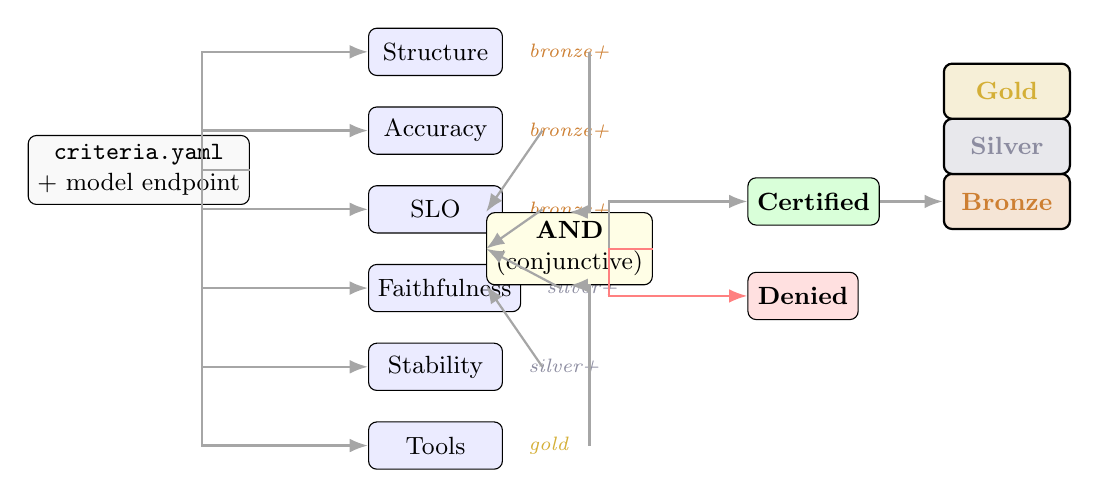
\begin{tikzpicture}[
    font=\small,
    node distance=0.6cm and 1.2cm,
    box/.style={draw, rounded corners=3pt, minimum width=2.0cm, minimum height=0.7cm, align=center, fill=gray!5},
    metric/.style={draw, rounded corners=3pt, minimum width=1.7cm, minimum height=0.6cm, align=center, fill=blue!8},
    pass/.style={draw, rounded corners=3pt, minimum width=1.4cm, minimum height=0.6cm, align=center, fill=green!15},
    fail/.style={draw, rounded corners=3pt, minimum width=1.4cm, minimum height=0.6cm, align=center, fill=red!12},
    tier/.style={draw, rounded corners=3pt, minimum width=1.6cm, minimum height=0.7cm, align=center, thick},
    arrow/.style={-Latex, thick, gray!70},
    failarrow/.style={-Latex, thick, red!50}
]
% Input
\node[box] (input) {\texttt{criteria.yaml}\\+ model endpoint};

% Metric families
\node[metric, right=1.5cm of input, yshift=1.5cm] (struct) {Structure};
\node[metric, right=1.5cm of input, yshift=0.5cm] (acc) {Accuracy};
\node[metric, right=1.5cm of input, yshift=-0.5cm] (slo) {SLO};
\node[metric, right=1.5cm of input, yshift=-1.5cm] (faith) {Faithfulness};
\node[metric, right=1.5cm of input, yshift=-2.5cm] (stab) {Stability};
\node[metric, right=1.5cm of input, yshift=-3.5cm] (tools) {Tools};

% Tier labels
\node[anchor=west, font=\scriptsize\itshape, text=bronze] at ([xshift=0.2cm]struct.east) {bronze+};
\node[anchor=west, font=\scriptsize\itshape, text=bronze] at ([xshift=0.2cm]acc.east) {bronze+};
\node[anchor=west, font=\scriptsize\itshape, text=bronze] at ([xshift=0.2cm]slo.east) {bronze+};
\node[anchor=west, font=\scriptsize\itshape, text=silver] at ([xshift=0.2cm]faith.east) {silver+};
\node[anchor=west, font=\scriptsize\itshape, text=silver] at ([xshift=0.2cm]stab.east) {silver+};
\node[anchor=west, font=\scriptsize\itshape, text=gold] at ([xshift=0.2cm]tools.east) {gold};

% Conjunction gate
\node[box, right=3.0cm of input, yshift=-1.0cm, minimum width=1.0cm, fill=yellow!10] (gate) {\textbf{AND}\\(conjunctive)};

% Verdict
\node[pass, right=1.2cm of gate, yshift=0.6cm] (certified) {\textbf{Certified}};
\node[fail, right=1.2cm of gate, yshift=-0.6cm] (denied) {\textbf{Denied}};

% Tier output
\node[tier, right=0.8cm of certified, fill=bronze!20] (bronze) {\textcolor{bronze}{\textbf{Bronze}}};
\node[tier, right=0.8cm of certified, yshift=0.7cm, fill=silver!20] (silver) {\textcolor{silver}{\textbf{Silver}}};
\node[tier, right=0.8cm of certified, yshift=1.4cm, fill=gold!20] (goldtier) {\textcolor{gold}{\textbf{Gold}}};

% Arrows
\draw[arrow] (input) -- ++(0.8,0) |- (struct.west);
\draw[arrow] (input) -- ++(0.8,0) |- (acc.west);
\draw[arrow] (input) -- ++(0.8,0) |- (slo.west);
\draw[arrow] (input) -- ++(0.8,0) |- (faith.west);
\draw[arrow] (input) -- ++(0.8,0) |- (stab.west);
\draw[arrow] (input) -- ++(0.8,0) |- (tools.west);

\draw[arrow] ([xshift=1.1cm]struct.east) |- (gate.north);
\draw[arrow] ([xshift=0.5cm]acc.east) -- (gate.north west);
\draw[arrow] ([xshift=0.5cm]slo.east) -- (gate.west);
\draw[arrow] ([xshift=0.5cm]faith.east) -- (gate.west);
\draw[arrow] ([xshift=0.5cm]stab.east) -- (gate.south west);
\draw[arrow] ([xshift=1.1cm]tools.east) |- (gate.south);

\draw[arrow] (gate) -- ++(0.5,0) |- (certified);
\draw[failarrow] (gate) -- ++(0.5,0) |- (denied);

\draw[arrow] (certified) -- (bronze);

\end{tikzpicture}
\end{adjustbox}
\caption{Certification evaluation flow. The \criteriayaml{} file and a model endpoint are the inputs. Each enabled metric family is evaluated independently, then results are combined through a conjunctive AND gate: \emph{all} families must pass for the target tier. The highest tier whose requirements are met determines the certification level.}
\label{fig:certification-flow}
\end{figure}

\subsection{Tier Definitions}

\begin{table}[t]
\centering
\caption{Certification tier requirements. Each higher tier includes all requirements of lower tiers. Thresholds shown are defaults; all are configurable per-deployment.}
\label{tab:tiers}
\small
\begin{tabular}{lccc}
\toprule
\textbf{Metric Family} & \textcolor{bronze}{\textbf{Bronze}} & \textcolor{silver}{\textbf{Silver}} & \textcolor{gold}{\textbf{Gold}} \\
\midrule
Structure: JSON Valid       & $\geq 0.95$ & $\geq 0.95$ & $\geq 0.99$ \\
Structure: Schema Compliant & $\geq 0.90$ & $\geq 0.90$ & $\geq 0.95$ \\
Accuracy (task-specific)    & required    & required    & required \\
SLO: latency tier           & meets tier  & meets tier  & meets tier \\
SLO: Success@SLO            & $\geq 0.70$ & $\geq 0.80$ & $\geq 0.90$ \\
\midrule
Faithfulness                & ---         & $\geq 0.80$ & $\geq 0.85$ \\
Stability (disagree@3)      & ---         & $\leq 0.15$ & $\leq 0.10$ \\
\midrule
Tools: Function Calling     & ---         & ---         & $\geq 0.85$\textsuperscript{*} \\
Tools: Routing              & ---         & ---         & $\geq 0.90$\textsuperscript{*} \\
\bottomrule
\multicolumn{4}{l}{\footnotesize \textsuperscript{*}Required only if \texttt{tools.enabled: true}.}
\end{tabular}
\end{table}

\subsubsection{\textcolor{bronze}{Bronze}: Structure + SLO}

Bronze is the minimum bar for production. It requires:
\begin{itemize}[leftmargin=12pt]
  \item At least 95\% of responses are valid JSON.
  \item At least 90\% of responses match the declared schema.
  \item The agent meets its declared SLO tier for latency.
  \item At least 70\% of responses are both correct and on-time (Success@SLO $\geq 0.70$).
\end{itemize}

Consider what this means against our data. Based on Paper~I results, only Llama-3.2-1B at the Batch tier would achieve Bronze among the 13 models we tested on consumer hardware. Not Silver. Not Gold. Bronze---the lowest tier---and only for one model. The deployment gap means that most models are \emph{not} production-ready under realistic constraints. The certification should reflect that reality rather than obscure it.

\subsubsection{\textcolor{silver}{Silver}: Bronze + Faithfulness + Stability}

Silver certification adds two dimensions that matter for user-facing applications:
\begin{itemize}[leftmargin=12pt]
  \item Faithfulness score $\geq 0.80$ (the agent does not fabricate information).
  \item Stability: disagreement@3 $\leq 0.15$ (the agent gives consistent answers).
\end{itemize}

Paper~II showed that faithfulness and stability are trainable properties: models that sustained GRPO training improvements typically achieved faithfulness above 0.8 and disagreement below 0.15. Paper~IV confirmed that these metrics are predictable from early training dynamics. Silver certification thus represents a model that has been deliberately optimized for production reliability.

\subsubsection{\textcolor{gold}{Gold}: Silver + Tools + Strict Compliance}

Gold certification is for mission-critical deployments. It raises all thresholds and adds tool use evaluation:
\begin{itemize}[leftmargin=12pt]
  \item JSON validity $\geq 0.99$ (near-zero structural failures).
  \item Success@SLO $\geq 0.90$ (nine out of ten requests succeed end-to-end).
  \item Faithfulness $\geq 0.85$ and disagreement@3 $\leq 0.10$.
  \item If tools are enabled: function calling $\geq 0.85$ and routing $\geq 0.90$.
  \item p99 (not just p95) latency compliance.
\end{itemize}

We designed Gold to be hard. Based on Paper~I data, achieving Gold at the Interactive tier would require models that do not yet exist in the open-weight ecosystem at consumer-hardware scale. This is intentional: Gold should represent genuine excellence, not a participation trophy.

\subsection{Evidence Mapping}

Table~\ref{tab:evidence} maps each metric family to the empirical evidence from Papers~I--V that motivates its inclusion and its default threshold.

\begin{table}[t]
\centering
\caption{Evidence base for each metric family and threshold. Each component of \criteriayaml{} traces to specific findings from the paper series.}
\label{tab:evidence}
\small
\begin{tabularx}{\linewidth}{lXl}
\toprule
\textbf{Metric} & \textbf{Evidence} & \textbf{Source} \\
\midrule
JSON Validity $\geq$0.95 & All 13 models exceed 99\%; threshold catches regressions & Paper~I \\
Schema Compliance $\geq$0.90 & Paper~I measured JSON validity ($\geq$99\%); compliance is stricter (correct fields, types). Threshold set below validity to allow field-level errors & Paper~I, V \\
Accuracy (varies) & Distribution across 5 task types; thresholds at median & Paper~I \\
Faithfulness $\geq$0.80 & Models below 0.8 fail to sustain training gains & Paper~II \\
disagree@3 $\leq$0.15 & Training reward stability component threshold & Paper~II, IV \\
Tool Calling $\geq$0.85 & Only 4B+ models learn T3; threshold above P1 median & Paper~I, II \\
SLO tiers & 2s/5s/30s from deployment research + P1 sensitivity & Paper~I, III \\
Success@SLO $\geq$0.80 & Compound metric; 0.80 is ambitious but achievable & Paper~III \\
\bottomrule
\end{tabularx}
\end{table}


% =============================================================================
\section{Evidence Base: How Papers I--V Support the Standard}
\label{sec:evidence}
% =============================================================================

We did not design \criteriayaml{} by committee. We derived it from empirical findings. This section maps each major result from the paper series to a specific component of the standard.

\subsection{Paper I: The Deployment Gap Demands Conjunctive Evaluation}

Paper~I~\citep{maloney2025deploymentgap} established that accuracy and SLO compliance are uncorrelated ($\rho = 0.09$, $p = 0.76$ at 2s). This single result motivates the entire \criteriayaml{} design philosophy: metrics must be evaluated \emph{conjunctively}. A model passes only if \emph{all} enabled metric families pass. The Success@SLO metric---counting only responses that are both correct and on-time---is the purest expression of this principle.

Paper~I also established the three SLO tiers used in the specification. Sensitivity analysis across deadline thresholds (2s, 5s, 10s) showed that the deployment gap is not an artifact of aggressive deadlines but a fundamental disconnect that persists across thresholds.

\subsection{Paper II: Capacity Thresholds Set Realistic Expectations}

Paper~II~\citep{maloney2025capacity} showed that the minimum model size for learning structured tasks is task-dependent. This finding directly shapes the tiered certification model. Bronze does not require tool calling precisely because Paper~II demonstrated that tool calling requires 4B+ models---excluding the smallest (and fastest) models that might otherwise achieve Bronze through speed alone.

The faithfulness threshold ($\geq$0.80) and stability threshold (disagree@3 $\leq$0.15) in Silver and Gold tiers come directly from Paper~II's composite reward function, where these values separated models that sustained training improvements from those that did not.

\subsection{Paper III: Three SLO Tiers Cover the Deployment Spectrum}

Paper~III~\citep{maloney2025agentslobench} formalized the evaluation protocol with three deployment tiers and established that per-request latency measurement (rather than aggregate percentile extrapolation) is essential for accurate Success@SLO computation. The specification inherits this methodology: SLO compliance is measured per-request with explicit warmup exclusion.

\subsection{Paper IV: Training Dynamics Enable Predictive Certification}

Paper~IV~\citep{maloney2025dynamics} demonstrated that training outcomes are predictable from early signals---the first 50 steps suffice. This opens the possibility of \emph{predictive certification}: a CI system could run abbreviated training and predict whether the full run would achieve the target tier. We list this as future work (Section~\ref{sec:future}), but the specification's design enables it.

Paper~IV reported 82.5\% overall early prediction accuracy from the first 50 training steps across 185 runs. The primary error mode was false positives---predicting sustained improvement when the actual trajectory was transient---occurring in approximately 12\% of cases. False negatives (predicting flat when the model eventually improved) were rarer, at approximately 5\%. For certification purposes, a false positive is the costlier error: it would lead a team to invest in full training only to discover the model cannot sustain gains. The asymmetric error profile suggests that predictive certification should use conservative thresholds, requiring stronger early signals before predicting a passing trajectory.

\subsection{Paper V: Production Validation}

Paper~V (forthcoming) will report on production deployments that apply the evaluation framework and the \criteriayaml{} specification to real-world workloads. Key questions that Paper~V is designed to answer include: (a)~whether the three SLO tiers (Interactive, Standard, Batch) cover the range of observed deployment scenarios or whether additional tiers are needed; (b)~whether the default thresholds are appropriate for production traffic patterns that differ from benchmark distributions; (c)~whether additional metric families---particularly Safety, Fairness, and Cost---are required for real deployments; and (d)~whether the certification tier achieved in offline evaluation predicts actual deployment success rates. The \criteriayaml{} specification is versioned at v0.1.0 precisely because these questions remain open; we expect Paper~V findings to motivate revisions in v0.2.0.


% =============================================================================
\section{Reference Implementation}
\label{sec:implementation}
% =============================================================================

\subsection{CLI Interface}

We built a Python CLI tool, \texttt{agentslo-eval}, that reads a \criteriayaml{} file and produces a certification verdict:

\begin{lstlisting}[language=bash, caption={CLI usage for \criteriayaml{} evaluation.}]
# Evaluate against criteria.yaml
$ agentslo-eval --config criteria.yaml --endpoint http://localhost:8000/v1

# Output:
# AgentSLO Evaluation Report
# ==========================
# Target tier: Silver
#
# Structure:
#   json_valid:       0.99 >= 0.95  PASS
#   schema_compliant: 0.94 >= 0.90  PASS
#
# Accuracy:
#   intent_classification: 0.87 >= 0.80  PASS
#   grounded_qa:           0.63 >= 0.60  PASS
#
# Faithfulness:        0.83 >= 0.80  PASS
#
# Stability:
#   disagreement@3:    0.11 <= 0.15  PASS
#
# SLO (Standard tier):
#   p95_ms:            3420 <= 5000  PASS
#   p99_ms:            6100 <= 8000  PASS
#   success@slo:       0.82 >= 0.80  PASS
#
# VERDICT: Silver CERTIFIED
\end{lstlisting}

\subsection{CI/CD Integration}

The tool is designed for CI pipelines. A non-zero exit code means certification failure---no parsing required:

\begin{lstlisting}[language=yaml, caption={GitHub Actions integration.}]
# .github/workflows/agent-eval.yml
name: Agent SLO Evaluation
on: [push, pull_request]

jobs:
  evaluate:
    runs-on: ubuntu-latest
    services:
      model-server:
        image: vllm/vllm-openai:latest
        ports: ["8000:8000"]
    steps:
      - uses: actions/checkout@v4
      - name: Install agentslo-eval
        run: pip install agentslo-eval
      - name: Run evaluation
        run: |
          agentslo-eval \
            --config criteria.yaml \
            --endpoint http://localhost:8000/v1 \
            --output-format json \
            --output-file results.json
      - name: Upload results
        uses: actions/upload-artifact@v4
        with:
          name: slo-eval-results
          path: results.json
\end{lstlisting}

\subsection{Output Formats}

The CLI produces three output formats:
\begin{itemize}[leftmargin=12pt]
  \item \textbf{Human-readable} (default): Formatted table with pass/fail indicators.
  \item \textbf{JSON}: Machine-parseable results for downstream tooling and experiment tracking (Weights \& Biases~\citep{wandb2020}, Weave~\citep{weave2024}).
  \item \textbf{Badge}: A Markdown or SVG badge indicating the achieved certification tier, suitable for model cards and README files.
\end{itemize}

As of this writing, the CLI exists as a working prototype. The companion repository includes a benchmark runner (\texttt{agent\_stable\_slo/bench/}) that implements the Structure and SLO metric families---per-request latency measurement and Success@SLO computation as described in Papers~I and~III. The remaining four families (Accuracy task dispatch, Faithfulness judge integration, Stability sampling, Tools evaluation) are under active development. We release the specification ahead of the complete implementation deliberately: community feedback on metric definitions and thresholds matters more than a finished tool.

\subsection{Integration with Experiment Tracking}

The JSON output format is designed to integrate with experiment tracking platforms. Each evaluation run produces a structured record containing:

\begin{lstlisting}[language=yaml, caption={JSON output schema (abbreviated).}]
{
  "version": "0.1.0",
  "timestamp": "2026-02-01T12:00:00Z",
  "config": { ... },           # criteria.yaml contents
  "results": {
    "structure": { "json_valid": 0.99, "schema_compliant": 0.94 },
    "accuracy": { "intent_classification": 0.87, "grounded_qa": 0.63 },
    "faithfulness": { "score": 0.83 },
    "stability": { "disagreement_at_3": 0.11 },
    "slo": { "p95_ms": 3420, "p99_ms": 6100, "success_at_slo": 0.82 }
  },
  "tier_target": "silver",
  "tier_achieved": "silver",
  "pass": true
}
\end{lstlisting}

This record can be logged to W\&B~\citep{wandb2020} or any experiment tracker that accepts JSON metrics. We envision three levels of integration with experiment tracking platforms: (1)~\emph{passive logging}, where the JSON output is uploaded as an artifact attached to a training or evaluation run; (2)~\emph{typed integration}, where the evaluation result is recognized as a first-class object---for example, a Weave~\citep{weave2024} evaluation type with structured fields for each metric family; and (3)~\emph{registry annotation}, where the certification tier is attached to a model version in a model registry, enabling queries such as ``show me all models that achieved Silver on Interactive tier.'' The reference implementation currently supports passive logging; deeper integration with specific platforms is planned for v0.2.0.

\subsection{Hardware-Diverse Validation}

Papers~I and~III taught us that SLO compliance is hardware-dependent. A model that meets the Interactive tier on an NVIDIA A100 may fail on an RTX~4090 or Apple M2~Max. ``Silver on datacenter GPUs'' is not a precise claim---it conflates the A100 (80\,GB HBM2e) with the H100 (80\,GB HBM3) despite their different memory bandwidth and inference throughput.

We therefore propose that certification be \emph{hardware-specific}. ``Silver on RTX~4090'' makes a precise, reproducible claim. The \texttt{metadata.hardware} field in \criteriayaml{} records the evaluation hardware, and we recommend that teams re-certify when deploying on different hardware classes. Validation across datacenter GPUs (A100, H100, L40S), consumer GPUs (RTX~4090, RTX~3090), and CPU/accelerator platforms (Apple M-series) is planned as part of the community validation process (Section~\ref{sec:validation}).


% =============================================================================
\section{Adoption Path}
\label{sec:adoption}
% =============================================================================

Standards fail when they demand too much too soon. \criteriayaml{} is designed for incremental adoption across four stages.

\subsection{Stage 1: Awareness (Week 1)}

A team creates a minimal \criteriayaml{} with only Structure and SLO enabled:

\begin{lstlisting}[language=yaml, caption={Minimal Bronze-tier \criteriayaml{} for initial adoption.}]
version: "0.1.0"
metadata:
  name: "my-agent"
  model: "llama-3.2-3b"
tier: bronze
structure:
  enabled: true
  json_valid:
    threshold: 0.95
    sample_size: 50
accuracy:
  enabled: true
  tasks:
    - name: "primary_task"
      type: "classification"
      dataset: "./tasks/eval.jsonl"
      threshold: 0.70
      metric: "exact_match"
slo:
  enabled: true
  tier: "standard"
  success_at_slo:
    threshold: 0.70
  measurement_requests: 50
\end{lstlisting}

Running \texttt{agentslo-eval} produces an immediate baseline. Most teams will discover their deployment gap at this stage.

\subsection{Stage 2: Integration (Weeks 2--4)}

The \criteriayaml{} file is committed to the repository and \texttt{agentslo-eval} is added to CI. Every pull request that modifies the agent configuration triggers an evaluation. The team begins tracking Success@SLO over time.

\subsection{Stage 3: Expansion (Months 1--3)}

The team enables Faithfulness and Stability families, targeting Silver certification. This typically requires changes to the agent: prompt engineering for faithfulness, temperature tuning for stability, or fine-tuning per Paper~II's methods.

\subsection{Stage 4: Maturity (Months 3+)}

The team enables Tools (if applicable) and targets Gold certification. At this stage, \criteriayaml{} becomes a contract between the agent team and the platform team: ``this agent is Gold-certified on Standard-tier SLOs.'' Certification is re-validated on every deployment.

Real-world adoption stories are essential for validating the four-stage adoption path. As the specification is currently at v0.1.0 draft stage, we have not yet collected independent adoption data. We invite teams deploying LLM agents in production---particularly those using LangChain~\citep{langchain2023}, CrewAI~\citep{crewai2024}, or AutoGen~\citep{autogen2023}---to pilot \criteriayaml{} and report their experience. Specifically, we seek teams at three deployment scales: (a)~a single-agent classification or extraction pipeline (targeting Bronze), (b)~a customer-facing QA or support agent requiring faithfulness guarantees (targeting Silver), and (c)~a multi-tool agent in a mission-critical workflow (targeting Gold). Pilot results will inform threshold adjustments in v0.2.0 and be reported in a follow-up publication.

\subsection{Model Hub Integration}

A natural extension is embedding \criteriayaml{} evaluation results in model hub pages. A HuggingFace model card could display:

\begin{quote}
\textbf{AgentSLO Certification:} \textcolor{silver}{\textbf{Silver}} on Standard tier (RTX 4090) \\
Success@SLO: 82\% | Faithfulness: 0.83 | Stability: 0.89
\end{quote}

The natural integration point is the Model Card metadata specification, which already supports structured fields for evaluation results. A \criteriayaml{} evaluation result could be embedded as a standard Model Card section---analogous to the existing ``Evaluation Results'' section but with machine-parseable certification status, tier, and hardware tag. An alternative is a dedicated evaluation tab on the model page, similar to the existing ``Spaces'' integration for interactive demos. Hardware-specific badges (e.g., \textcolor{silver}{\textbf{Silver}} on RTX~4090, \textcolor{bronze}{\textbf{Bronze}} on M2~Max) would require extending the Model Card schema to support multiple evaluation configurations per model. We view this integration as a community-driven effort and welcome discussion with model hub maintainers.

\subsection{Serving Layer Integration}

For local serving tools (LM Studio, Ollama, vLLM~\citep{kwon2023vllm}), the \criteriayaml{} evaluation could be triggered automatically when a model is loaded:

\begin{lstlisting}[language=bash]
# Hypothetical: LM Studio integration
$ lms eval --criteria criteria.yaml --model llama-3.2-3b
# Runs evaluation and displays certification status in the UI
\end{lstlisting}

We recommend an opt-in model: users trigger evaluation explicitly rather than running it automatically on model load. Automatic evaluation would add latency to the model-loading experience and require bundling task datasets with the serving tool---a non-trivial distribution problem. Instead, serving tools could expose a ``Run SLO Eval'' button or CLI flag that invokes the reference implementation against the currently loaded model. A ``quick mode'' that evaluates only Structure and SLO families on a minimal sample (50 requests) could provide a Bronze-tier assessment in under two minutes on consumer hardware, making it practical for interactive use.


% =============================================================================
\section{Community Process}
\label{sec:community}
% =============================================================================

A standard is only as good as the community that adopts it. We propose an RFC-style process for evolving \criteriayaml{}, modeled on the Python Enhancement Proposal (PEP) process and the OpenAPI Specification's evolution.

\subsection{Governance Structure}

We propose a three-tier governance structure modeled on successful open-specification projects:

\begin{itemize}[leftmargin=12pt]
  \item \textbf{Steering Committee} (5--7 members): Sets strategic direction and approves specification-level changes. The committee must include at least one representative from each of four constituencies: (a)~an academic institution with active research in LLM evaluation, (b)~an infrastructure provider offering GPU-diverse compute, (c)~an agent framework development team, and (d)~a team operating LLM agents in production. The initial committee will be formed from respondents to an open call for participation, published alongside the v0.1.0 specification draft.

  \item \textbf{Working Groups}: Metric-family-specific groups---Structure WG, Accuracy WG, Faithfulness WG, Tools WG, Stability WG, and SLO WG---that propose threshold changes, validate new measurement methods, and review RFCs within their domain. Each working group requires a minimum of three members from at least two organizations.

  \item \textbf{Community Contributors}: Anyone can submit an RFC via pull request to the specification repository. Working groups triage and review submissions; the Steering Committee makes final accept/reject decisions.
\end{itemize}

The governance structure is itself a proposal. We recognize that standards governance requires sustained institutional commitment, and we do not presume that the initial author can unilaterally convene a representative committee. The open call for participation will be published alongside this paper and the specification repository, with the goal of seating the initial Steering Committee within six months of publication.

\subsection{RFC Process}

\begin{enumerate}[leftmargin=16pt]
  \item \textbf{Draft}: Author submits an RFC as a GitHub pull request against the specification repository.
  \item \textbf{Discussion}: 30-day public comment period. Comments are threaded on the PR.
  \item \textbf{Review}: The relevant Working Group reviews the RFC and produces a recommendation (accept, revise, reject).
  \item \textbf{Decision}: The Steering Committee votes. Simple majority for metric-family changes; two-thirds majority for specification-level changes (new families, tier modifications).
  \item \textbf{Implementation}: Accepted RFCs are implemented in the reference CLI before the specification version is bumped.
\end{enumerate}

The proposed timeline for the v0.1.0 release is:

\begin{itemize}[leftmargin=12pt]
  \item \textbf{Q1 2026}: Circulate draft specification and this paper to potential partner organizations for preliminary feedback.
  \item \textbf{Q2 2026}: Open a 60-day RFC period for the v0.1.0 specification. All RFCs submitted as pull requests to the specification repository.
  \item \textbf{Q3 2026}: Incorporate feedback, conduct validation with at least three independent teams (Section~\ref{sec:validation}), and finalize threshold defaults.
  \item \textbf{Q4 2026}: Release v0.1.0 specification with reference CLI implementation, JSON Schema, and evaluation protocol documentation.
\end{itemize}

This timeline is aspirational. The critical dependency is community engagement: without three independent validation teams, the specification cannot advance beyond draft status. We prefer a delayed but well-validated v0.1.0 over a premature release that undermines trust in the standard.

\subsection{Versioning}

The specification follows Semantic Versioning 2.0.0:
\begin{itemize}[leftmargin=12pt]
  \item \textbf{MAJOR} (1.0.0\,$\to$\,2.0.0): Breaking changes to the schema. Existing \criteriayaml{} files may not be valid.
  \item \textbf{MINOR} (0.1.0\,$\to$\,0.2.0): New metric families or tier modifications. Existing files remain valid.
  \item \textbf{PATCH} (0.1.0\,$\to$\,0.1.1): Threshold defaults, documentation, reference implementation fixes.
\end{itemize}


% =============================================================================
\section{Validation Requirements}
\label{sec:validation}
% =============================================================================

A proposal is not a standard. Before \criteriayaml{} earns that title, it must be validated independently. We define four requirements:

\subsection{Requirement 1: Reproducibility}

At least three independent teams must be able to install the reference implementation, create a \criteriayaml{} file, and produce evaluation results that are consistent with each other (within measurement noise) when evaluating the same model on the same hardware.

We seek three validation teams meeting the following diversity criteria: (a)~different organizations (no two teams from the same company), (b)~different primary use cases (e.g., customer support, research evaluation, tool-using agents), and (c)~different hardware (at least one datacenter GPU, one consumer GPU, and one non-NVIDIA platform). The validation protocol requires each team to independently install the reference implementation, create a \criteriayaml{} file for their deployment, evaluate at least two models, and report whether the certification results are reproducible and meaningful. An open call for validation partners will be published alongside the specification repository.

\subsection{Requirement 2: Discrimination}

The certification tiers must meaningfully discriminate between models. Specifically: (a) not all models should achieve the same tier, (b) tier should correlate with an independent measure of production success, and (c) the tier ordering should be robust to reasonable threshold perturbations ($\pm$10\%).

Based on Paper~I data (13 models, 29{,}900 predictions on consumer hardware), we can project tier assignments under default thresholds. At the Interactive tier (2s), 12 of 13 models achieved 0\% Success@SLO, meaning none would achieve even Bronze certification---the deployment gap in its starkest form. At the Batch tier (30s), model rankings shift substantially: the smallest models (Llama-3.2-1B, Qwen2.5-3B) become competitive because their speed advantage converts directly into SLO compliance. Paper~II's 11 trained models show improvement: models that sustained GRPO training gains (sustained curve type) achieved faithfulness above 0.80 and disagreement below 0.15, meeting the Silver tier requirements on those dimensions. The tier distribution is sensitive to the Success@SLO threshold: relaxing the Bronze threshold from 0.70 to 0.60 would admit 2--3 additional models at the Standard tier, while tightening Gold from 0.90 to 0.95 would likely exclude all models in our evaluation. This sensitivity analysis will be published in full alongside the specification.

\subsection{Requirement 3: Hardware Diversity}

Certification results must be validated across at least three hardware configurations: datacenter GPU (A100 or H100), consumer GPU (RTX 4090), and CPU/Apple Silicon (M2/M3).

The author's empirical work in Papers~I--IV was conducted on an NVIDIA RTX 4090 (consumer GPU), providing the baseline for consumer hardware validation. Datacenter GPU validation (A100, H100) and Apple Silicon validation (M2/M3 Max via MLX or llama.cpp backends) require community partners. We invite infrastructure providers and research labs with access to these platforms to participate in the hardware diversity validation. The key hypothesis to test is whether tier assignments are stable across hardware classes or whether hardware-specific certification is strictly necessary---Paper~I evidence suggests the latter.

\subsection{Requirement 4: Framework Diversity}

The specification must work with at least two different agent frameworks (e.g., LangChain + CrewAI) and two different serving backends (e.g., vLLM + Ollama).

Framework integration testing will proceed in three phases: (1)~vLLM~\citep{kwon2023vllm} with LangChain~\citep{langchain2023}, the most common production pairing, validating that the OpenAI-compatible API interface works end-to-end with \texttt{agentslo-eval}; (2)~Ollama with direct HTTP API calls, testing the specification on the most popular local serving tool without a framework abstraction layer; and (3)~LM Studio with CrewAI~\citep{crewai2024}, testing multi-agent orchestration on a desktop-oriented serving backend. Each phase must demonstrate that the same \criteriayaml{} file produces consistent certification results (within measurement noise) regardless of the framework and serving combination used.


% =============================================================================
\section{Limitations and Future Work}
\label{sec:future}
% =============================================================================

\subsection{Current Limitations}

\textbf{Single-author evidence base.} We are honest about this limitation: Papers~I--V represent a single research program. The findings span 13 models from 8 vendors across 4 countries, but the experimental design, metric choices, and threshold selections reflect one perspective. Community validation (Section~\ref{sec:validation}) is essential.

\textbf{Safety and fairness are absent.} The current specification does not include safety (toxicity, bias, harmful content) or fairness (demographic parity, equalized odds) metric families. This is a deliberate scope limitation---safety evaluation is a complex domain that deserves its own specification~\citep{weidinger2022taxonomy,bommasani2021foundation}---but it means \criteriayaml{} certification does not imply the agent is safe or fair.

\textbf{Closed-source models.} The specification assumes the evaluator has direct access to the model (via an API endpoint). For closed-source models behind rate-limited APIs, SLO measurement reflects the API provider's infrastructure rather than the model's intrinsic capabilities. The specification currently does not distinguish between ``model is slow'' and ``API is slow.''

\textbf{Multi-agent systems.} The specification evaluates a single agent in isolation. Multi-agent systems (orchestrators, tool chains, ensembles) have emergent properties that single-agent evaluation cannot capture. A natural extension is hierarchical certification: each agent in a pipeline maintains its own \criteriayaml{}, and a pipeline-level specification defines end-to-end SLO budgets that are decomposed across agents (e.g., a 5-second pipeline SLO might allocate 2 seconds to the router agent and 3 seconds to the worker agent). This decomposition pattern is well-established in microservice SLO management and translates directly to multi-agent systems. We defer this extension to a future RFC.

\textbf{Cost metrics.} Papers~II and~IV included token cost ($C$) in the reward function, but the current specification does not include a Cost metric family. We considered adding Cost as a seventh metric family but concluded that cost is better treated as a metadata annotation rather than a certification requirement. The reason is that cost depends on pricing models that vary by provider, change over time, and differ between self-hosted and API-accessed deployments. A model that costs \$0.001 per request on self-hosted vLLM may cost \$0.01 through a managed API---the model has not changed, but the cost has. We recommend recording cost-per-request in the evaluation output metadata and leaving cost thresholds to organizational procurement decisions rather than embedding them in a universal specification.

\subsection{Future Work}

\textbf{Predictive certification.} Paper~IV showed that training outcomes are predictable from early signals. A natural extension is a ``fast-track'' certification mode that runs 50 training steps and predicts the achievable tier without full evaluation. This could reduce certification time from hours to minutes.

\textbf{Continuous certification.} The current specification is designed for point-in-time evaluation. Production systems need continuous monitoring: is the agent \emph{still} meeting its certification requirements? Integration with observability platforms (Datadog, Grafana, W\&B~\citep{wandb2020}) could enable continuous certification with alerting on tier degradation.

\textbf{Domain-specific extensions.} Healthcare, finance, and legal applications have domain-specific requirements (HIPAA compliance, regulatory accuracy, citation requirements) that the generic specification cannot capture. Domain-specific \criteriayaml{} extensions could be defined as RFC-approved supplements.

\textbf{Multilingual evaluation.} Papers~I--V used English-only tasks. The specification does not address language-specific evaluation or multilingual agents. Extending \criteriayaml{} to multilingual settings raises two questions: first, whether metric thresholds should vary by language (accuracy on low-resource languages is typically lower than on English for equivalent models), and second, whether the SLO tiers should account for tokenization differences (languages with larger token-to-character ratios may systematically require more inference time). We recommend that multilingual task sets be contributed as community RFCs with language-specific threshold recommendations.

\textbf{Safety metric family.} The most important omission. A future version should include a Safety family with configurable toxicity, bias, and harmful content metrics. This will require collaboration with the AI safety community and alignment with frameworks like NIST AI RMF~\citep{nist2023airmf} and the EU AI Act~\citep{euaiact2024}.


% =============================================================================
\section{Conclusion}
\label{sec:conclusion}
% =============================================================================

The LLM agent ecosystem is building on sand. Teams select models based on accuracy benchmarks that do not predict deployment success ($\rho = 0.09$), evaluate quality dimensions in isolation when production requires them in conjunction, and discover the deployment gap only after investing weeks in integration. There is no shared language for ``production-ready.''

This paper proposes \criteriayaml{} as that shared language. The specification encodes six metric families---Structure, Accuracy, Faithfulness, Tools, Stability, and SLO compliance---into a declarative, machine-readable file that CI/CD systems can enforce. Three certification tiers (Bronze, Silver, Gold) allow incremental adoption. Every component traces to empirical evidence from five prior papers spanning 13 models, 42{,}900 evaluations, and 185 training runs.

The proposal is deliberately incomplete. The threshold defaults need community validation. The safety and fairness dimensions need dedicated working groups. The governance structure needs real people, not placeholders. The specification itself needs at least three independent teams to implement, test, and critique it before it earns the title of ``standard.''

But the need is real. Every team deploying an LLM agent faces the same questions: Is the structure valid? Are the answers correct? Is the model making things up? Does it give consistent answers? Can it call tools? Does it respond in time? \criteriayaml{} provides a way to answer all of these questions with a single command, produce a reusable certification, and communicate the result to stakeholders.

We close with an invitation. The specification, reference implementation, and RFC process are open. We explicitly invite infrastructure providers, experiment tracking platforms, model hubs, local serving tools, and agent framework teams to participate in the v0.1.0 review. Submit an RFC. Run the evaluation on your models. Tell us where the thresholds are wrong, where the metric families are incomplete, where the specification does not fit your deployment reality. A standard that reflects one researcher's perspective is a draft; a standard that reflects the community's collective experience is a foundation. The deployment gap is real, the fragmentation is measurable, and the solution must be shared.

The specification, reference implementation, and community process are available at:
\begin{center}
\texttt{https://github.com/neuralift/agentslo-spec} \\
\texttt{https://agentslo.dev/criteria/v0.1.0/}
\end{center}


% =============================================================================
% ACKNOWLEDGMENTS
% =============================================================================
\section*{Acknowledgments}

The empirical work underlying this specification was conducted across Papers~I--IV with support from the University of New Hampshire. The open-weight models used in our evaluations were made available by Meta, Google, Alibaba (Qwen team), Microsoft, Mistral AI, the Technology Innovation Institute, 01.AI, and OpenAI. Experiment tracking was facilitated by Weights \& Biases. Local model serving relied on LM Studio and vLLM. We thank the developers of these tools for building the infrastructure that makes independent LLM evaluation research possible. We also thank the anonymous reviewers and early readers whose feedback shaped the specification design.


% =============================================================================
% BIBLIOGRAPHY
% =============================================================================
\bibliographystyle{plainnat}
\bibliography{refs}


% =============================================================================
% APPENDIX
% =============================================================================
\appendix

\section{JSON Schema for \criteriayaml{} Validation}
\label{app:jsonschema}

The following is an abbreviated JSON Schema for validating \criteriayaml{} files. The full schema (approximately 280 lines) is hosted at the URL below and is used by the reference implementation for validation at parse time.

\begin{lstlisting}[language={}, caption={Abbreviated JSON Schema for \criteriayaml{} (key sections).}]
{
  "$schema": "https://json-schema.org/draft/2020-12/schema",
  "$id": "https://agentslo.dev/criteria/v0.1.0/schema.json",
  "title": "criteria.yaml",
  "description": "Production-readiness specification for LLM agents",
  "type": "object",
  "required": ["version", "metadata", "tier"],
  "properties": {
    "version": {
      "type": "string",
      "pattern": "^[0-9]+\\.[0-9]+\\.[0-9]+$"
    },
    "metadata": {
      "type": "object",
      "required": ["name", "model"],
      "properties": {
        "name": { "type": "string" },
        "model": { "type": "string" },
        "framework": { "type": "string" },
        "serving": { "type": "string" },
        "hardware": { "type": "string" },
        "author": { "type": "string", "format": "email" },
        "created": { "type": "string", "format": "date" }
      }
    },
    "tier": {
      "type": "string",
      "enum": ["bronze", "silver", "gold"]
    },
    "structure": {
      "type": "object",
      "properties": {
        "enabled": { "type": "boolean" },
        "json_valid": {
          "type": "object",
          "properties": {
            "threshold": { "type": "number", "minimum": 0, "maximum": 1 },
            "sample_size": { "type": "integer", "minimum": 1 }
          }
        },
        "schema_compliant": {
          "type": "object",
          "properties": {
            "threshold": { "type": "number", "minimum": 0, "maximum": 1 },
            "schema_ref": { "type": "string" }
          }
        }
      }
    },
    "slo": {
      "type": "object",
      "properties": {
        "enabled": { "type": "boolean" },
        "tier": { "enum": ["interactive", "standard", "batch"] },
        "latency": {
          "type": "object",
          "patternProperties": {
            "^(interactive|standard|batch)$": {
              "type": "object",
              "properties": {
                "p95_ms": { "type": "integer", "minimum": 0 },
                "p99_ms": { "type": "integer", "minimum": 0 }
              }
            }
          }
        },
        "success_at_slo": {
          "type": "object",
          "properties": {
            "threshold": { "type": "number", "minimum": 0, "maximum": 1 }
          }
        }
      }
    }
  }
}
\end{lstlisting}

The full JSON Schema---including definitions for the \texttt{accuracy}, \texttt{faithfulness}, \texttt{tools}, and \texttt{stability} families, along with tier-conditional validation rules---is available at:
\begin{center}
\texttt{https://agentslo.dev/criteria/v0.1.0/schema.json}
\end{center}


\section{Mapping to Existing Standards}
\label{app:mapping}

Table~\ref{tab:mapping} maps \criteriayaml{} concepts to analogous concepts in existing standards.

\begin{table}[ht]
\centering
\caption{Concept mapping between \criteriayaml{} and existing standards.}
\label{tab:mapping}
\small
\begin{tabularx}{\linewidth}{lXX}
\toprule
\textbf{\criteriayaml{}} & \textbf{Analogue} & \textbf{Standard} \\
\midrule
\texttt{version} & Schema version & OpenAPI Specification~\citep{openapi2021} \\
\texttt{metadata} & Model Card header & Model Cards~\citep{mitchell2019modelcards} \\
\texttt{tier} & Submission category & MLPerf~\citep{reddi2020mlperf} \\
\texttt{structure} & Output format & JSON Schema~\citep{jsonschema2020} \\
\texttt{accuracy} & Task benchmarks & HELM~\citep{liang2023helm} \\
\texttt{slo} & Latency requirements & MLPerf Inference~\citep{reddi2020mlperf} \\
\texttt{faithfulness} & Grounding & RAGAS~\citep{es2023ragas} \\
Certification badge & Model Card annotation & Model Cards~\citep{mitchell2019modelcards} \\
RFC process & PEP process & Python (PEP~1) \\
\bottomrule
\end{tabularx}
\end{table}


\section{Full Evaluation Protocol}
\label{app:protocol}

The following protocol is designed to be reproducible by an independent team without access to the reference implementation source code.

\begin{enumerate}[leftmargin=16pt]
  \item \textbf{Hardware setup and warmup.} Record the GPU model, VRAM, driver version, and serving backend (vLLM, Ollama, LM Studio, etc.). Load the model and send \texttt{warmup\_requests} requests (default: 10) that are excluded from all measurements. Warmup ensures that model weights are loaded into GPU memory and any JIT compilation or KV cache allocation has completed.

  \item \textbf{Task sampling.} For each task defined in the \texttt{accuracy} section, load the dataset and draw a stratified sample of size \texttt{sample\_size} (default: 100). Stratification ensures that all label classes (for classification) or difficulty levels (for QA) are represented proportionally. If the dataset is smaller than \texttt{sample\_size}, use the full dataset and note the reduced sample in the output.

  \item \textbf{Latency measurement.} Measure wall-clock time per request from the moment the HTTP request is sent to the moment the complete response is received. This is end-to-end latency including tokenization, inference, and detokenization but excluding network round-trip time to remote APIs. For local serving (vLLM, Ollama, LM Studio), the evaluator and model server must run on the same machine or same local network to minimize network variance. Record each request's latency in milliseconds; compute p95 and p99 from the empirical distribution.

  \item \textbf{Structure evaluation.} For each response, attempt JSON parsing. Record success/failure for \texttt{json\_valid}. For responses that parse as valid JSON, validate against the declared JSON Schema (\texttt{schema\_ref}). Record success/failure for \texttt{schema\_compliant}. Compute fractions over all \texttt{measurement\_requests}.

  \item \textbf{Accuracy evaluation.} For each task, compare the model's response to the ground truth using the declared metric (\texttt{exact\_match}, \texttt{f1}, or custom). For classification tasks, extract the predicted label from the structured response. For QA tasks, extract the answer span. Compute the aggregate metric over all samples.

  \item \textbf{Faithfulness evaluation} (Silver and Gold tiers). For each sample in the faithfulness evaluation set, send the model's response and the input context to the judge model with the following prompt template: ``Given the context below, determine whether every claim in the response is supported by the context. Return a score between 0.0 (no claims supported) and 1.0 (all claims supported).'' Record the judge's score per sample; compute the mean. The judge model must be specified in the \texttt{faithfulness.judge\_model} field.

  \item \textbf{Stability evaluation} (Silver and Gold tiers). For each prompt in the stability evaluation set, generate $k$ independent responses at the declared temperature (\texttt{stability.temperature}, default: 0.7). Compare the $k$ responses using the task-appropriate metric (exact match for classification, token-level F1 for QA). A prompt is ``disagreed'' if any pair of the $k$ responses differs. Compute \texttt{disagreement@k} as the fraction of prompts with disagreement.

  \item \textbf{Success@SLO computation.} For each request, the response is ``successful'' if and only if it is (a)~correct according to the accuracy metric \emph{and} (b)~delivered within the declared latency tier's p95 threshold. Compute \texttt{success\_at\_slo} as the fraction of successful requests over all \texttt{measurement\_requests}.

  \item \textbf{Statistical requirements.} Report 95\% bootstrap confidence intervals (1,000 resamples) for all aggregate metrics. The minimum sample size for SLO measurement is 100 requests; for faithfulness and stability, 50 samples. Results with sample sizes below these minimums should be flagged as provisional.

  \item \textbf{Edge case handling.} Timeouts (no response within $2\times$ the tier's p99 threshold) are counted as failures for both accuracy and SLO. Malformed responses (non-JSON when JSON is expected) are counted as structure failures and accuracy failures. Empty responses are counted as failures across all metric families.
\end{enumerate}


\section{Comparison of Evaluation Frameworks}
\label{app:comparison}

Table~\ref{tab:comparison} compares \criteriayaml{} against existing evaluation frameworks across six dimensions relevant to production deployment decisions.

\begin{table}[ht]
\centering
\caption{Comparison of evaluation frameworks across production-relevant dimensions. \cmark{} = supported, \pmark{} = partial, --- = not supported.}
\label{tab:comparison}
\small
\begin{adjustbox}{max width=\linewidth}
\begin{tabular}{lcccccc}
\toprule
\textbf{Framework} & \textbf{Accuracy} & \textbf{Structure} & \textbf{Latency} & \textbf{Pass/Fail} & \textbf{CI/CD} & \textbf{Hardware} \\
\midrule
HELM~\citep{liang2023helm}                & \cmark & ---    & ---    & ---    & ---    & ---    \\
JSONSchemaBench~\citep{geng2025jsonschemabench} & ---    & \cmark & ---    & ---    & ---    & ---    \\
Chatbot Arena~\citep{chiang2024chatbot}    & \pmark & ---    & ---    & ---    & ---    & ---    \\
RAGAS~\citep{es2023ragas}                  & \pmark & ---    & ---    & ---    & ---    & ---    \\
LM Eval Harness~\citep{gao2023lmeval}     & \cmark & ---    & ---    & ---    & \pmark & ---    \\
OpenCompass~\citep{opencompass2023}         & \cmark & \pmark & ---    & ---    & \pmark & ---    \\
Inspect~\citep{ukaisi2024inspect}          & \cmark & \pmark & ---    & \pmark & \cmark & ---    \\
BIG-Bench~\citep{srivastava2023bigbench}   & \cmark & ---    & ---    & ---    & ---    & ---    \\
\midrule
\criteriayaml{} (this work)                & \cmark & \cmark & \cmark & \cmark & \cmark & \cmark \\
\bottomrule
\end{tabular}
\end{adjustbox}
\end{table}

The distinguishing feature of \criteriayaml{} is the conjunction of all six dimensions: no existing framework combines accuracy evaluation with structured output validation, latency-aware SLO compliance, conjunctive pass/fail verdicts, CI/CD integration patterns, and hardware-specific certification. Each existing framework excels in its primary dimension---HELM for breadth of accuracy benchmarks, JSONSchemaBench for schema compliance rigor, Inspect for composable evaluation pipelines---but none produces the deployment-ready certification that \criteriayaml{} targets.


\end{document}
